\begin{SCn}

\scnsectionheader{\currentname}

\scnstartsubstruct

\scnheader{Предметная область и онтология действий,  задач, планов, протоколов и методов, реализуемых ostis-системой в ее памяти, а также внутренних агентов, выполняющих эти действия}
\scniselement{предметная область}
\scnsdmainclass{действие в sc-памяти;абстрактный sc-агент;sc-агент}
\scnsdclass{абстрактный sc-агент, не реализуемый на Языке SCP;абстрактный sc-агент, реализуемый на Языке SCP;Абстрактный программный sc-агент;неатомарный абстрактный sc-агент;атомарный абстрактный sc-агент;платформенно-независимый абстрактный sc-агент;платформенно-зависимый абстрактный sc-агент;внутренний абстрактный sc-агент;эффекторный абстрактный sc-агент;рецепторный абстрактный sc-агент;абстрактный sc-агент, не реализуемый на Языке SCP;абстрактный sc-агент, реализуемый на Языке SCP;
абстрактный sc-агент интерпретации scp-программ;абстрактный программный sc-агент;
абстрактный программный sc-агент, реализуемый на Языке SCP;абстрактный sc-метаагент;sc-агент;активный sc-агент;описание поведения sc-агента;тип блокировки;полная блокировка;блокировка на любое изменение;блокировка на удаление}
\scnsdrelation{декомпозиция абстрактного sc-агента*;ключевые sc-элементы sc-агента*;программа sc-агента*;первичное условие инициирования*;условие инициирования и результат*;блокировка*}

\scnheader{обработка информации в ostis-системах}
\scnrelfromlist{принципы, лежащие в основе}{
	\scnfileitem{В основе решателя задач каждой \textit{ostis-системы} лежит многоагентная система, агенты которой взаимодействуют между собой \uline{только}(!) через общую для них \textit{sc-память} посредством спецификации в этой памяти выполняемых ими \textit{действий в sc-памяти}. При этом пользователи \textit{ostis-системы} также считаются агентами этой системы. Кроме того, \textit{sc-агенты} делятся на внутренние, рецепторные и эффекторные. Взаимодействие между агентами через общую \textit{sc-память} сводится к следующим видам действий:
	\begin{scnenumerate}
		\item К использованию общедоступной для соответствующей группы sc-агентов части хранимой базы знаний;
		\item К формированию (генерации) новых фрагментов базы знаний и/или к корректировке (редактированию) каких-либо фрагментов доступной части базы знаний;
		\item К интеграции (погружению) новых и/или обновленных фрагментов в состав доступной части базы знаний;
	\end{scnenumerate}\\
	Подчеркнем, что sc-агенты не общаются между собой напрямую путем отправки сообщений, как это делается в большинстве современных подходов к построению многоагентных систем. Кроме того, sc-агенты имеют доступ к общей для них базе знаний за счет чего гарантируется семантическая совместимость (взаимопонимание) между агентами, включая и пользователей ostis-систем};
	\scnfileitem{Пользователь \textit{ostis-системы} не может сам непосредственно выполнить какое-либо действие в sc-памяти, но он может средствами пользовательского интерфейса инициировать построение (генерацию, формирование в \textit{sc-памяти}) \textit{sc-текста}, являющегося спецификацией \textit{действия в sc-памяти}, выполняемого либо одним \textit{атомарным sc-агентом} за один акт, либо одним \textit{атомарным sc-агентом} за несколько актов, либо коллективом \textit{sc-агентов} (\textit{неатомарным sc-агентом}). В спецификации каждого такого \textit{действия в sc-памяти}, инициированного пользователем, этот пользователь указывается как заказчик этого действия. Таким образом, пользователь \textit{ostis-системы} дает поручения (задания, команды) \textit{sc-агентам} этой системы на выполнение различных специфицируемых им действий в \textit{sc-памяти}.};
	\scnfileitem{Каждый \textit{sc-агент}, выполняя некоторое \textit{действие в sc-памяти}, должен "помнить"{}, что \textit{sc-память}, над которой он работает, является общим ресурсом не только для него, но и для всех остальных \textit{sc-агентов}, работающих над этой же \textit{sc-памятью}. Поэтому \textit{sc-агент} должен соблюдать определенную этику поведения в коллективе таких \textit{sc-агентов}, которая должна минимизировать помехи, которые он создает другим \textit{sc-агентам}.};
	\scnfileitem{Деятельность каждого агента \textit{ostis-системы} дискретна и представляет собой множество элементарных действий (актов). При этом при выполнении каждого акта агент может устанавливать блокировки нескольких типов на фрагменты базы знаний. Указанные блокировки позволяют запретить другим агентам изменять указанный фрагмент базы знаний или вообще сделать его "невидимым"{} для других агентов. Блокировки устанавливаются самим агентом при выполнении соответствующего акта и снимаются им же на последнем этапе выполнения этого акта или раньше, если это возможно.};
	\scnfileitem{Если некий \textit{sc-агент} выполняет некоторое \textit{действие в sc-памяти}, то он на время выполнения этого действия может:
	\begin{scnenumerate}
		\item Запретить другим \textit{sc-агентам} изменять состояние некоторых sc-элементов, хранимых в \textit{sc-памяти} -- удалять их, изменять тип;
		\item Запретить другим \textit{sc-агентам} добавлять или удалять элементы некоторых множеств, обозначаемых соответствующими \textit{sc-узлами};
		\item Запретить другим \textit{sc-агентам} доступ на просмотр некоторых \textit{sc-элементов}, то есть эти \textit{sc-элементы} становятся полностью "невидимыми"{} (полностью заблокированными) для других \textit{sc-агентов} но только на время выполнения соответствующего действия.
	\end{scnenumerate}\\
	Указанные блокировки должны быть полностью сняты до завершения выполнения соответствующего действия. Подчеркнем, что число \textit{sc-элементов}, блокируемых на время выполнения некоторого действия, в основном входят атомарные и неатомарные связки, и не должны входить \textit{sc-узлы}, обозначающие бесконечные классы каких-либо сущностей, и, тем более, sc-узлы, обозначающие различные понятия (ключевые классы различных предметных областей).\\
	Этичное (неэгоистичное) поведение \textit{sc-агента}, касающееся блокировки \textit{sc-элементов} (то есть ограничения к ним доступа другим \textit{sc-агентам}) предполагает соблюдение следующих правил:
	\begin{scnenumerate}
		\item Не следует блокировать больше \textit{sc-элементов}, чем это необходимо для решения задачи;
		\item Как только для какого-либо \textit{sc-элемента} необходимость его блокировки отпадает до завершения выполнения соответствующего действия, этот \textit{sc-элемент} желательно сразу деблокировать (снять блокировку);
	\end{scnenumerate}\\
	Для того, чтобы \textit{sc-агент} имел возможность работы с каким-либо произвольным \textit{sc-элементом}, он должен либо убедиться в том, что этот \textit{sc-элемент} не входит во фрагмент базы знаний, входящий в \textit{полную блокировку}, либо убедиться в том, что эта блокировка не установлена самим этим агентом.\\
	Особой группой полностью заблокированных \textit{sc-элементов} (на время выполнения действия \textit{sc-агентом}) являются вспомогательные \textit{sc-элементы} ("леса"{}), создаваемые только на время выполнения этого действия. Эти sc-элементы в конце выполнения действия должны не деблокироваться, а удаляться.};
	\scnfileitem{Если \textit{действие в sc-памяти}, выполняемое \textit{sc-агентом}, завершилось (т.е. стало прошлой сущностью), то \textit{sc-агент} оформляет результат этого \textit{действия}, указывая (1) удаленные \textit{sc-элементы} и (2) сгенерированные sc-элементы. Это необходимо, если по каким-либо причинам придется сделать откат этого \textit{действия}, т.е возвратиться к состоянию базы знаний до выполнения указанного \textit{действия}.}
}

\scnsegmentheader{Понятие действия в sc-памяти}
\scnstartsubstruct

\scnheader{действие в sc-памяти}
\scnidtf{внутреннее действие ostis-системы}
\scnidtf{действие, выполняемое в sc-памяти}
\scnidtf{действие, выполняемое в абстрактной унифицированной семантической памяти}
\scnidtf{действие, выполняемое машиной обработки знаний ostis-системы}
\scnidtf{действие, выполняемое агентом или коллективом агентов ostis-системы}
\scnidtf{информационный процесс над базой знаний, хранимой в sc-памяти}
\scnidtf{процесс решения информационной задачи в sc-памяти}
\scnsubset{процесс в sc-памяти}
\scnexplanation{Каждое \textbf{\textit{действие в sc-памяти}} обозначает некоторое преобразование, выполняемое некоторым \textit{sc-агентом} (или коллективом \textit{sc-агентов}) и ориентированное на преобразование \textit{sc-памяти}. Спецификация действия после его выполнения может быть включена в протокол решения некоторой задачи. 

Преобразование состояния базы знаний включает, в том числе и информационный поиск, предполагающий (1) локализацию в базе знаний ответа на запрос, явное выделение структуры ответа и (2) трансляцию ответа на некоторый внешний язык.

Во множество \textbf{\textit{действий в sc-памяти}} входят знаки действий самого различного рода, семантика каждого из которых зависит от конкретного контекста, т.е. ориентации действия на какие-либо конкретные объекты и принадлежности действия какому-либо конкретному классу действий.

Следует четко отличать:
\begin{scnitemize}
\item Каждое конкретное \textbf{\textit{действие в sc-памяти}}, представляющее собой некоторый переходный процесс, переводящий sc-память из одного состояния в другое;
\item Каждый тип \textbf{\textit{действий в sc-памяти}}, представляющий собой некоторый класс однотипных (в том или ином смысле) действий;
\item sc-узел, обозначающий некоторое конкретное \textbf{\textit{действие в sc-памяти}};
\item sc-узел, обозначающий структуру, которая является описанием, спецификацией, заданием, постановкой соответствующего действия.
\end{scnitemize}
}
\scnsuperset{действие в sc-памяти, инициируемое вопросом}
\scnsuperset{действие редактирования базы знаний ostis-системы}
\scnsuperset{действие установки режима ostis-системы}
\scnsuperset{действие редактирования файла, хранимого в sc-памяти}
\scnsuperset{действие интерпретации программы, хранимой в sc-памяти}

\scnheader{действие в sc-памяти, инициируемое вопросом}
\scnidtf{действие, направленное на формирование ответа на поставленный вопрос}
\scnsuperset{действие. cформировать заданный файл}
\scnsuperset{действие. cформировать заданную структуру}
\scnaddlevel{1}
	\scnsuperset{действие. верифицировать заданную структуру}
	\scnaddlevel{1}
		\scnsuperset{действие. установить истинность или ложность указываемого логического высказывания}
		\scnsuperset{действие. установить корректность или некорректность указываемой структуры}
		\scnsuperset{действие. сформировать структуру, описывающую некорректности, имеющиеся в указываемой структуре}
	\scnaddlevel{-1}
	\scnsuperset{действие. уточнить тип заданного sc-элемента}
	\scnaddlevel{1}
		\scnsuperset{действие. установить позитивность/негативность указываемой sc-дуги принадлежности или непринадлежности}
	\scnaddlevel{-1}
	\scnsuperset{действие. сформировать семантическую окрестность}
	\scnaddlevel{1}
		\scnsuperset{действие. сформировать полную семантическую окрестность указываемой сущности}
		\scnsuperset{действие. сформировать базовую семантическую окрестность указываемой сущности}
		\scnsuperset{действие. сформировать частную семантическую окрестность указываемой сущности}
	\scnaddlevel{-1}
	\scnsuperset{действие. сформировать структуру, описывающую связи между указываемыми сущностями}
	\scnaddlevel{1}
		\scnsuperset{действие. сформировать структуру, описывающую сходства указываемых сущностей}
		\scnsuperset{действие. сформировать структуру, описывающую различия указываемых сущностей}
	\scnaddlevel{-1}
	\scnsuperset{действие. сформировать структуру, описывающую способ решения указываемой задачи}
	\scnsuperset{действие. сформировать план генерации ответа на указанный вопрос}
	\scnsuperset{действие. сформировать протокол выполнения указываемого действия}
	\scnsuperset{действие. сформировать обоснование корректности указываемого решения}
	\scnsuperset{действие. верифицировать обоснование корректности указываемого решения}
	\scnsuperset{действие, направленное на установление темпоральных характеристик указываемой сущности}
	\scnsuperset{действие, направленное на установление пространственных характеристик указываемой сущности}
\scnaddlevel{-1}

\scnheader{действие редактирования базы знаний}
\scnsuperset{действие. изменить направление указанной sc-дуги}
\scnsuperset{действие. исправить ошибки в заданной структуре}
\scnsuperset{действие. преобразовать указанную структуру в соответствии с указанным правилом}
\scnsuperset{действие. отождествить два указанных sc-элемента}
\scnsuperset{действие. включить множество}
\scnaddlevel{1}
	\scnidtf{сделать все элементы множества \textbf{\textit{Si}} явно принадлежащими множеству \textbf{\textit{Sj}}, то есть сгенерировать соответствующие sc-дуги принадлежности}
\scnaddlevel{-1}
\scnsuperset{действие генерации sc-элементов}
\scnaddlevel{1}
	\scnsuperset{действие генерации, одним из аргументов которого является некоторая обобщенная структура}
	\scnaddlevel{1}
		\scnsuperset{действие. сгенерировать структуру, изоморфную указываемому образцу}
	\scnaddlevel{-1}
	\scnsuperset{действие. сгенерировать sc-элемент указанного типа}
	\scnaddlevel{1}
		\scnsuperset{действие. сгенерировать sc-коннектор указанного типа}
		\scnsuperset{действие. сгенерировать sc-узел указанного типа}
	\scnaddlevel{-1}
	\scnsuperset{действие. сгенерировать файл с заданным содержимым}
	\scnsuperset{действие. установить указанный файл в качестве основного идентификатора указанного sc-элемента для указанного внешнего языка}
\scnaddlevel{-1}
\scnsuperset{действие. обновить понятия}
\scnaddlevel{1}
	\scnidtf{действие. заменить неосновные понятия на их определения через основные понятия}
\scnaddlevel{-1}
\scnsuperset{действие. интегрировать информационную конструкцию в текущее состояние базы знаний}
\scnaddlevel{1}
	\scnsuperset{действие. интегрировать содержимое указанного файла в текущее состояние базы знаний}
	\scnaddlevel{1}
		\scnsuperset{действие. протранслировать содержимое указанного файла в sc-память}
	\scnaddlevel{-1}
	\scnsuperset{действие. интегрировать указанную структуру в текущее состояние базы знаний}
\scnaddlevel{-1}
\scnsuperset{действие. дополнить описание прошлого состояния ostis-системы}
\scnaddlevel{1}
	\scnsuperset{действие. дополнить структуру, описывающую историю эволюции ostis-системы}
	\scnsuperset{действие. дополнить структуру, описывающую историю эксплуатации ostis-системы}
\scnaddlevel{-1}

\scnsuperset{действие удаления sc-элементов}
\scnaddlevel{1}
    \scnsuperset{действие. удалить указанные sc-элементы}
   	\scnaddlevel{1}
	\scnsuperset{действие. удалить sc-элементы, входящие в состав указанной структуры и не являющиеся ключевыми узлами каких-либо sc-агентов}
	\scnaddlevel{-1}
\scnresetlevel

\scnheader{действие. отождествить два указанных sc-элемента}
\scnidtf{действие. совместить два указанных sc-элемента}
\scnidtf{действие. склеить два указанных sc-элемента}
\scnsubdividing{действие. физически отождествить два указанных sc-элемента;действие. логически отождествить два указанных sc-элемента}

\scnheader{действие. отождествить два указанных sc-элемента}
\scnexplanation{Каждое \textbf{\textit{действие. отождествить два указанных sc-элемента}} может быть выполнено как \textit{действие. физически отождествить два указанных sc-элемента} или \textit{действие. логически отождествить два указанных sc-элемента}. В случае логического отождествления в протоколе деятельности агентов сохраняется само действие с его спецификацией, включающей обязательное указание того, какие элементы были сгенерированы, а какие удалены. В случае физического отождествления протокол действия не сохраняется.}

\scnheader{действие. обновить понятия}
\scnidtf{действие. заменить некоторое множество понятий на другое множество понятий}
\scnexplanation{Каждое \textbf{\textit{действие. обновить понятия}} обозначает переход от какой-то группы понятий, использовавшихся ранее, к другой группе понятий, которые будут использоваться вместо первых, и станут \textit{основными понятиями}.
В общем случае \textbf{\textit{действие. обновить понятия}} состоит из следующих этапов:

\begin{scnitemize}
    \item Определить заменяемые понятия на основе заменяющих;
    \item Внести соответствующие изменения в программы sc-агентов, ключевыми узлами которых являются обновляемые понятия;
    \item Заменить все конструкции в базе знаний, содержащие заменяемые понятия, в соответствии с определениями этих понятий через заменяющие их понятия;
    \item При необходимости,\textit{ sc-элементы}, обозначающие замененные таким образом понятия, могут быть полностью выведены из текущего состояния базы знаний.
\end{scnitemize}

Первым аргументом (входящим в знак \textit{действия} под атрибутом \textit{1’}) \textbf{\textit{действия. обновить понятия}} является знак множества \textit{sc-узлов}, обозначающих заменяемые понятия, вторым (входящим в знак \textit{действия} под атрибутом \textit{2’}) - знак множества \textit{sc-узлов}, обозначающих заменяющие понятия. В общем случае любое или оба этих множества могут быть \textit{синглетонами}.}

\scnheader{действие. удалить указанные sc-элементы}
\scnsubdividing{действие. физически удалить указанные sc-элементы;действие. логически удалить указанные sc-элементы}
\scnexplanation{Каждое \textbf{\textit{действие. удалить указанные sc-элементы}} может быть выполнено как \textit{действие. физически удалить указанные sc-элементы} или \textit{действие. логически удалить указанные sc-элементы}. В случае логического удаления в протоколе деятельности агентов сохраняется само действие с его спецификацией, включающей обязательное указание того, какие элементы были удалены, т.е. по сути, элементы просто исключаются из текущего состояния базы знаний. В случае физического удаления протокол действия не сохраняется.

В случае удаления какого-либо \textit{sc-элемента}, инцидентные ему \textit{связки}, в том числе \textit{sc-коннекторы}, также удаляются.}

\scnheader{действие. интегрировать указанную структуру в текущее состояние базы знаний}
\scnexplanation{Для того, чтобы выполнить \textbf{\textit{действие. интегрировать указанную структуру в текущее состояние базы знаний}}, необходимо склеить \textit{sc-элементы}, входящие в интегрируемую \textit{структуру} с синонимичными им \textit{sc-элементами}, входящими в текущее состояние базы знаний, заменить неиспользуемые (например, устаревшие) понятия, входящие в интегрируемую \textit{структуру}, на используемые (т.е. заменить неиспользуемые понятия на их определения через используемые), явно включить все элементы интегрируемой \textit{структуры} в число элементов утвержденной части базы знаний и явно включить все элементы интегрируемой \textit{структуры} в число элементов одного из атомарных разделов утвержденной части базы знаний.}

\scnheader{действие интерпретации программы, хранимой в sc-памяти}
\scnsuperset{действие интерпретации scp-программы}

\scnheader{задача, решаемая в sc-памяти}
\scnsubset{задача}
\scnidtf{спецификация действия, выполняемого в sc-памяти}
\scnidtf{структура, являющая таким описанием (постановкой, заданием) соответствующего действия в sc-памяти, которое обладает достаточной полнотой для выполения указанного действия}
\scnidtf{семантическая окрестность некоторого действия в sc-памяти, обеспечивающая достаточно полное задание этого действия}

\scnheader{класс действий}
\scnsuperset{класс действий в sc-памяти}
\scnaddlevel{1}
	\scnrelto{семейство подмножеств}{действие в sc-памяти}
\scnaddlevel{-1}
\scnsubdividing{класс логически атомарных действий\\
	\scnaddlevel{1}
		\scnidtf{класс автономных действий}
	\scnaddlevel{-1};	
	класс логически неатомарных действий\\
	\scnaddlevel{1}
	\scnidtf{класс неавтономных действий}
	\scnaddlevel{-1}}

\scnheader{класс логически атомарных действий}
\scnexplanation{Каждое \textit{действие}, принадлежащее некоторому конкретному \textit{классу логически атомарных действий}, обладает двумя необходимыми свойствами:
\begin{scnitemize}
	\item выполнение действия не зависит от того, является ли указанное действие частью декомпозиции более общего действия. При выполнении данного действия также не должен учитываться тот факт, что данное действие предшествует каким-либо другим действиям или следует за ними (что явно указывается при помощи отношения \textit{последовательность действий*});
	\item указанное действие должно представлять собой логически целостный акт преобразования, например, в семантической памяти. Такое действие по сути является транзакцией, т. е. результатом такого преобразования становится новое состояние преобразуемой системы, а выполняемое действие должно быть либо выполнено полностью, либо не выполнено совсем, частичное выполнение не допускается. 
\end{scnitemize}

В то же время логическая атомарность не запрещает декомпозировать выполняемое действие на более частные, каждое из которых, в свою очередь, также будет являться логически атомарным.}
\scnsuperset{класс логически атомарных действий в sc-памяти}
\scnaddlevel{1}
	\scnexplanation{На логически атомарные действия предлагается делить всю деятельность, направленную на решение каких-либо задач ostis-системой. Соответственно \textit{решатель задач ostis-системы} предлагается делить на компоненты, соответствующие таким \textit{классам логически атомарных действий в sc-памяти}, что является основой для обеспечения его \textit{модифицируемости}.}
\scnaddlevel{-1}

\scnendstruct 

\scnsegmentheader{Понятие sc-агента и абстрактного sc-агента}

\scnstartsubstruct

\scnheader{sc-агент}
\scnidtf{единственный вид \textit{субъектов}, выполняющих преобразования в \textit{\textit{sc-памяти}}}
\scnidtf{\textit{субъект}, способный выполнять \textit{действия в sc-памяти}, принадлежащие некоторому определенному \textit{классу логически атомарных действий}}
\scnexplanation{Логическая атомарность выполняемых sc-агентом действий предполагает, что каждый sc-агент реагирует на соответствующий ему класс ситуаций и/или событий, происходящих в sc-памяти, и осуществляет определенное преобразование sc-текста, находящегося в семантической окрестности обрабатываемой ситуации и/или события. При этом каждый sc-агент в общем случае не имеет информацию о том, какие еще sc-агенты в данный момент присутствуют в системе и осуществляет взаимодействие в другими sc-агентами исключительно посредством формирования некоторых конструкций (как правило – спецификаций действий) в общей sc-памяти. Таким сообщением может быть, например, вопрос, адресованный другим sc-агентам в системе (заранее не известно, каким конкретно), или ответ на поставленный другими sc-агентами вопрос (заранее не известно, каким конкретно). Таким образом, каждый sc-агент в каждый момент времени контролирует только фрагмент базы знаний в контексте решаемой данным агентом задачи, состояние всей остальной базы знаний в общем случае непредсказуемо для sc-агента.}

\scnheader{абстрактный sc-агент}
\scnnote{Поскольку предполагается, что копии одного и того же \textit{sc-агента} или функционально эквивалентные \textit{sc-агенты} могут работать в разных ostis-системах, будучи при этом физически разными sc-агентами, то целесообразно рассматривать свойства и классификацию не sc-агентов, а классов функционально эквивалентных sc-агентов, которые будем называть \textit{абстрактными sc-агентами}.}
\scnexplanation{Под \textbf{\textit{абстрактным sc-агентом}} понимается некоторый класс функционально эквивалентных \textit{sc-агентов}, разные экземпляры (т.е. представители) которого могут быть реализованы по-разному.

Каждый \textbf{\textit{абстрактный sc-агент}} имеет соответствующую ему спецификацию. В спецификацию каждого \textbf{\textit{абстрактного sc-агента}} входит:
\begin{scnitemize}
    \item указание ключевых \textit{sc-элементов} этого \textit{sc-агента}, т.е. тех \textit{sc-элементов}, хранимых в \textit{sc-памяти}, которые для данного \textit{sc-агента} являются «точками опоры»;
    \item формальное описание условий инициирования данного \textit{sc-агента}, т.е. тех \textit{ситуация} в \textit{sc-памяти}, которые инициируют деятельность данного \textit{sc-агента};
    \item формальное описание первичного условия инициирования данного \textit{sc-агента}, т.е. такой ситуации в \textit{sc-памяти}, которая побуждает \textit{sc-агента} перейти в активное состояние и начать проверку наличия своего полного условия инициирования (для \textit{внутренних абстрактных sc-агентов});
    \item строгое, полное, однозначно понимаемое описание деятельности данного \textit{sc-агента}, оформленное при помощи каких-либо понятных, общепринятых средств, не требующих специального изучения, например на естественном языке.
    \item описание результатов выполнения данного \textit{sc-агента}.
\end{scnitemize}
}
\scnsubdividing{неатомарный абстрактный sc-агент;атомарный абстрактный sc-агент}
\scnsubdividing{внутренний абстрактный sc-агент;эффекторный абстрактный sc-агент;рецепторный абстрактный sc-агент}
\scnsubdividing{абстрактный sc-агент, не реализуемый на Языке SCP;абстрактный sc-агент, реализуемый на Языке SCP}
\scnsubdividing{абстрактный sc-агент интерпретации scp-программ;абстрактный программный sc-агент;абстрактный sc-метаагент}
\scnsubdividing{платформенно-зависимый абстрактный sc-агент\\
\scnaddlevel{1}
\scnsuperset{абстрактный sc-агент, не реализуемый на Языке SCP}
\scnaddlevel{-1}
;платформенно-независимый абстрактный sc-агент}

\scnheader{абстрактный sc-агент, не реализуемый на Языке SCP}
\scnidtf{абстрактный sc-агент, который не может быть реализован на платформенно-независимом уровне}
\scnsubdividing{эффекторный абстрактный sc-агент;рецепторный абстрактный sc-агент
;абстрактный sc-агент интерпретации scp-программ}

\scnheader{абстрактный sc-агент, реализуемый на Языке SCP}
\scnidtf{абстрактный sc-агент, который может быть реализован на платформенно-независимом уровне}
\scnsubdividing{абстрактный sc-метаагент;абстрактный программный sc-агент, реализуемый на Языке SCP}

\scnheader{абстрактный программный sc-агент}
\scnsubdividing{эффекторный абстрактный sc-агент;рецепторный абстрактный sc-агент
;абстрактный программный sc-агент, реализуемый на Языке SCP}

\scnheader{неатомарный абстрактный sc-агент}
\scnexplanation{Под \textbf{\textit{неатомарным абстрактным sc-агентом}} понимается \textit{абстрактный sc-агент}, который декомпозируется на коллектив более простых \textit{абстрактных sc-агентов}, каждый из которых в свою очередь может быть как \textit{атомарным абстрактным sc-агентом}, так и \textbf{\textit{неатомарным абстрактным sc-агентом}}. При этом в каком либо варианте \textit{декомпозиции абстрактного sc-агента*} дочерний \textbf{\textit{неатомарный абстрактный sc-агент}} может стать \textit{атомарным абстрактным sc-агентом}, и реализовываться соответствующим образом.}

\scnheader{атомарный абстрактный sc-агент}
\scnexplanation{Под \textbf{\textit{атомарным абстрактным sc-агентом}} понимается \textit{абстрактный sc-агент}, для которого уточняется платформа его реализации, т.е. существует соответствующая связка отношения \textit{программа sc-агента*}.}
\scnsubdividing{платформенно-независимый абстрактный sc-агент;платформенно-зависимый абстрактный sc-агент}

\scnheader{платформенно-независимый абстрактный sc-агент}
\scnexplanation{К \textbf{\textit{платформенно-независимым абстрактным sc-агентам}} относят \textit{атомарные абстрактные sc-агенты}, реализованные на базовом языке программирования Технологии OSTIS, т.е. на \textit{Языке SCP}.

При описании \textbf{\textit{платформенно-независимых абстрактных sc-агентов}} под платформенной независимостью понимается платформенная независимость с точки зрения Технологии OSTIS, т.е реализация на специализированном языке программирования, ориентированном на обработку семантических сетей (\textit{Языке SCP}), поскольку \textit{атомарные sc-агенты}, реализованные на указанном языке могут свободно переноситься с одной платформы интерпретации \textit{sc-моделей} на другую. При этом языки программирования, традиционно считающиеся платформенно-независимыми в данном случае не могут считаться таковыми.

Существуют \textit{sc-агенты}, которые принципиально не могут быть реализованы на платформенно-независимом уровне, например, собственно \textit{sc-агенты} интерпретации \textit{sc-моделей} или рецепторные и эффекторные \textit{sc-агенты}, обеспечивающие взаимодействие с внешней средой.}

\scnheader{платформенно-зависимый абстрактный sc-агент}
\scnexplanation{К \textbf{\textit{платформенно-зависимым абстрактным sc-агентам}} относят \textit{атомарные абстрактные sc-агенты}, реализованные ниже уровня sc-моделей, т.е. не на \textit{Языке SCP}, а на каком-либо другом языке описания программ.

Существуют \textit{sc-агенты}, которые принципиально должны быть реализованы на платформенно-зависимом уровне, например, собственно \textit{sc-агенты} интерпретации \textit{sc-моделей} или рецепторные и эффекторные \textit{sc-агенты}, обеспечивающие взаимодействие с внешней средой.}

\scnheader{внутренний абстрактный sc-агент}
\scnexplanation{Каждый \textbf{\textit{внутренний абстрактный sc-агент}} обозначает класс \textit{sc-агентов}, которые реагируют на события в \textit{sc-памяти} и осуществляют преобразования исключительно в рамках этой же \textit{sc-памяти}.}

\scnheader{эффекторный абстрактный sc-агент}
\scnexplanation{Каждый \textbf{\textit{эффекторный абстрактный sc-агент}} обозначает класс \textit{sc-агентов}, которые реагируют на события в \textit{sc-памяти} и осуществляют преобразования во внешней относительно данной \textit{ostis-системы} среде.}

\scnheader{рецепторный абстрактный sc-агент}
\scnexplanation{Каждый \textbf{\textit{рецепторный абстрактный sc-агент}} обозначает класс \textit{sc-агентов}, которые реагируют на события во внешней относительно данной \textit{ostis-системы} среде и осуществляют преобразования в памяти данной системы.}

\scnheader{абстрактный sc-агент, не реализуемый на Языке SCP}
\scnexplanation{Каждый \textbf{\textit{абстрактный sc-агент, не реализуемый на Языке SCP}} должен быть реализован на уровне платформы интерпретации sc-моделей, в том числе, аппаратной. К таким \textit{абстрактным sc-агентам} относятся абстрактные sc-агенты интерпретации scp-программ, а также эффекторные и рецепторные абстрактные sc-агенты.}

\scnheader{абстрактный sc-агент, реализуемый на Языке SCP}
\scnexplanation{Каждый \textbf{\textit{абстрактный sc-агент, реализуемый на Языке SCP}} может быть реализован на Языке SCP, то есть платформенно-независимом уровне, но при необходимости, может реализовываться и на уровне платформы, например, с целью повышения производительности.}

\scnheader{абстрактный sc-агент интерпретации scp-программ}
\scnexplanation{К \textbf{\textit{абстрактным sc-агентам интерпретации scp-программ}} относятся не реализуемые на платформенно-независимом уровне \textit{абстрактные sc-агенты}, обеспечивающие интерпретацию \textit{scp-программ} и \textit{scp-метапрограмм}, в том числе создание \textit{scp-процессов}, собственно интерпретацию \textit{scp-операторов}, а также другие вспомогательные действия. По сути, агенты данного класса обеспечивают работу sc-агентов более высоких уровней (программных sc-агентов и sc-метаагентов), реализованных на Языке SCP, в частности, обеспечивают соблюдение указанными агентами общих принципов синхронизации.}

\scnheader{абстрактный программный sc-агент}
\scnexplanation{К \textbf{\textit{абстрактным программным sc-агентам}} относятся все \textit{абстрактные sc-агенты}, обеспечивающие основной функционал системы, то есть ее возможность решать те или иные задачи. Агенты данного класса должны работать в соответствии с общими принципами синхронизации деятельности субъектов в sc-памяти.}

\scnheader{абстрактный программный sc-агент, реализуемый на Языке SCP}

\scnheader{абстрактный sc-метаагент}
\scnexplanation{Задачей \textbf{\textit{абстрактных sc-метаагентов}} является координация деятельности \textit{абстрактных программных sc-агентов}, в частности, решение проблемы взаимоблокировок. Агенты данного класса могут быть реализованы на Языке SCP, однако для синхронизации их деятельности используются другие принципы, соответственно, для реализации таких агентов требуется Язык SCP другого уровня, типология операторов которого полностью аналогична типологии scp-операторов, однако эти операторы имеют другую операционную семантику, учитывающую отличия в принципах синхронизации (работы с \textit{блокировками*}). Программы такого языка будем называть \textit{scp-метапрограммами}, соответствующие им \textit{процессы в sc-памяти} – \textit{scp-метапроцессами}, операторы – \textit{scp-метаоператорами}.}

\scnheader{декомпозиция абстрактного sc-агента*}
\scniselement{отношение декомпозиции}
\scnexplanation{Отношение \textbf{\textit{декомпозиции абстрактного sc-агента*}} трактует \textit{неатомарные абстрактные sc-агенты} как коллективы более простых \textit{абстрактных sc-агентов}, взаимодействующих через \textit{sc-память}.

Другими словами, \textbf{\textit{декомпозиция абстрактного sc-агента*}} на \textit{абстрактные sc-агенты} более низкого уровня уточняет один из возможных подходов к реализации этого \textit{абстрактного sc-агента} путем построения коллектива более простых \textit{абстрактных sc-агентов}.}

\scnheader{sc-агент}
\scnidtf{агент над sc-памятью}
\scnsubset{субъект}
\scnrelfrom{семейство подмножеств}{абстрактный sc-агент}
\scnexplanation{Под \textbf{\textit{sc-агентом}} понимается конкретный экземпляр (с теоретико-множественной точки зрения - элемент) некоторого \textit{атомарного абстрактного sc-агента}, работающий в какой-либо конкретной интеллектуальной системе.

Таким образом, каждый \textit{sc-агент} - это субъект, способный выполнять некоторый класс однотипных действий либо только над \textit{sc-памятью}, либо над sc-памятью и внешней средой (для эффекторных \textit{sc-агентов}). Каждое такое действие инициируется либо состоянием или ситуацией в sc-памяти, либо состоянием или ситуацией во внешней среде (для рецепторных sc-агентов-датчиков),  соответствующей условию инициирования \textit{атомарного абстрактного sc-агента}, экземпляром которого является заданный \textit{sc-агент}. В данном случае можно провести аналогию между принципами объектно-ориентированного программирования, рассматривая \textit{атомарный абстрактный sc-агент} как класс, а конкретный \textit{sc-агент} – как экземпляр, конкретную имплементацию этого класса.

Взаимодействие \textit{sc-агентов} осуществляется только через \textit{sc-память}. Как следствие, результатом работы любого \textit{sc-агента} является некоторое изменение состояния \textit{sc-памяти}, т.е. удаление либо генерация каких-либо \textit{sc-элементов}.

В общем случае один \textit{sc-агент} может явно передать управление другому \textit{sc-агенту}, если этот \textit{sc-агент} априори известен. Для этого каждый \textit{sc-агент} в \textit{sc-памяти} имеет обозначающий его \textit{sc-узел}, с которым можно связать конкретную ситуацию в текущем состоянии базы знаний, которую инициируемый \textit{sc-агент} должен обработать.

Однако далеко не всегда легко определить того \textit{sc-агента}, который должен принять управление от заданного \textit{sc-агента}, в связи с чем описанная выше ситуация возникает крайне редко. Более того, иногда условие инициирования \textit{sc-агента} является результатом деятельности непредсказуемой группы \textit{sc-агентов}, равно как и одна и та же конструкция может являться условием инициирования целой группы \textit{sc-агентов}.

При этом общаются через \textit{sc-память} не \textit{программы sc-агентов*}, а сами описываемые данными программами \textit{sc-агенты}.

В процессе работы \textit{sc-агент} может сам для себя порождать вспомогательные \textit{sc-элементы}, которые сам же удаляет после завершения акта своей деятельности (это вспомогательные \textit{структуры}, которые используются в качестве "информационных лесов"{} только в ходе выполнения соответствующего акта деятельности и после завершения этого акта удаляются).}

\scnheader{активный sc-агент}
\scnsubset{sc-агент}
\scnexplanation{Под \textbf{\textit{активным sc-агентом}} понимается \textit{sc-агент} ostis-системы, который реагирует на события, соответствующие его условию инициирования, и, как следствие, его \textit{первичному условию инициирования*}. Не входящие во множество \textbf{\textit{активных sc-агентов}} \textit{sc-агенты} не реагируют ни на какие события в \textit{sc-памяти}.}

\scnheader{ключевые sc-элементы sc-агента*}
\scnexplanation{Связки отношения \textbf{\textit{ключевые sc-элементы sc-агента*}} связывают между собой \textit{sc-узел}, обозначающий \textit{абстрактный sc-агент} и \textit{sc-узел}, обозначающий множество \textit{sc-элементов}, которые являются ключевыми для данного \textit{абстрактного sc-агента}, то данные \textit{sc-элементы} явно упоминаются в рамках программ, реализующих данный \textit{абстрактный sc-агент}.}

\scnheader{программа sc-агента*}
\scnexplanation{Связки отношения \textbf{\textit{программа sc-агента*}} связывают между собой \textit{sc-узел}, обозначающий \textit{атомарный абстрактный sc-агент} и \textit{sc-узел}, обозначающий множество программ, реализующих указанный \textit{атомарный абстрактный sc-агент}. В случае \textit{платформенно-независимого абстрактного sc-агента} каждая связка отношения \textit{программа sc-агента*} связывает \textit{sc-узел}, обозначающий указанный \textit{абстрактный sc-агент} с множеством \textit{scp-программ}, описывающих деятельность данного \textit{абстрактного sc-агента}. Данное множество содержит одну \textit{агентную scp-программу}, и произвольное количество (может быть, и ни одной) \textit{scp-программ}, которые необходимы для выполнения указанной \textit{агентной scp-программы}.

В случае \textit{платформенно-зависимого абстрактного sc-агента} каждая связка отношения \textit{программа sc-агента*} связывает \textit{sc-узел}, обозначающий указанный \textit{абстрактный sc-агент} с множеством файлов, содержащих исходные тексты программы на некотором внешнем языке программирования, реализующей деятельность данного \textit{абстрактного sc-агента}.}

\scnheader{первичное условие инициирования*}
\scnexplanation{Связки отношения \textbf{\textit{первичное условие инициирования*}} связывают между собой \textit{sc-узел}, обозначающий \textit{абстрактный sc-агент} и бинарную ориентированную пару, описывающую первичное условие инициирования данного \textit{абстрактного sc-агента}, т.е. такой спецификацию \textit{ситуации} в \textit{sc-памяти}, возникновение которой побуждает \textit{sc-агента} перейти в активное состояние и начать проверку наличия своего полного условия инициирования.

Первым компонентом данной ориентированной пары является знак некоторого класса \textit{элементарных событий в sc-памяти*}, например, \textit{событие добавления sc-дуги, выходящей из заданного sc-элемента*}.

Вторым компонентом данной ориентированной пары является произвольный в общем случае \textit{sc-элемент}, с которым непосредственно связан указанный тип события в \textit{sc-памяти}, т.е., например, \textit{sc-элемент}, из которого выходит либо в который входит генерируемая либо удаляемая \textit{sc-дуга}, либо \textit{файл}, содержимое которого было изменено.

После того, как в \textit{sc-памяти} происходит некоторое событие, активизируются все \textit{активные sc-агенты}, \textbf{\textit{первичное условие инициирования*}} которых соответствует произошедшему событию.}

\scnheader{условие инициирования и результат*}
\scnexplanation{Связки отношения \textbf{\textit{условие инициирования и результат*}} связывают между собой \textit{sc-узел}, обозначающий \textit{абстрактный sc-агент} и бинарную ориентированную пару, связывающую условие инициирования данного \textit{абстрактного sc-агента} и результаты выполнения данного экземпляров данного \textit{sc-агента} в какой-либо конкретной системе.

Указанную ориентированную пару можно рассматривать как логическую связку импликации, при этом на \textit{sc-переменные}, присутствующие в обеих частях связки, неявно накладывается квантор всеобщности, на \textit{sc-переменные}, присутствующие либо только в посылке, либо только в заключении неявно накладывается квантор существования.

Первым компонентом указанной ориентированной пары является логическая формула, описывающая условие инициирования описываемого \textit{абстрактного sc-агента}, то есть конструкции, наличие которой в \textit{sc-памяти} побуждает \textit{sc-агент} начать работу по изменению состояния \textit{sc-памяти}. Данная логическая формула может быть как атомарной, так и неатомарной, в которой допускается использование любых связок логического языка.

Вторым компонентом указанной ориентированной пары является логическая формула, описывающая возможные результаты выполнения описываемого абстрактного \textit{sc-агента}, то есть описание произведенных им изменений состояния \textit{sc-памяти}. Данная логическая формула может быть как атомарной, так и неатомарной, в которой допускается использование любых связок логического языка.}

\scnheader{описание поведения sc-агента}
\scnsubset{семантическая окрестность}
\scnexplanation{\textbf{\textit{описание поведения sc-агента}} представляет собой \textit{семантическую окрестность}, описывающую деятельность \textit{sc-агента} до какой-либо степени детализации, однако такое описание должно быть строгим, полным и однозначно понимаемым. Как любая другая \textit{семантическая окрестность}, \textbf{\textit{описание поведения sc-агента}} может быть протранслировано на какие-либо понятные, общепринятые средства, не требующие специального изучения, например на естественный язык.\\
Описываемый \textit{абстрактный sc-агент} входит в соответствующее \textbf{\textit{описание поведения sc-агента}} под атрибутом \textit{ключевой sc-элемент'}.}

\scnendstruct 

\scnsegmentheader{Принципы синхронизации деятельности sc-агентов}

\scnstartsubstruct

\scnheader{процесс в sc-памяти}
\scnnote{Понятия \textit{действие в sc-памяти}, и \textit{процесс в sc-памяти} (информационный процесс, выполняемый агентом в семантической памяти), являются синонимичными, поскольку все процессы, протекающие в sc-памяти, являюся осознанными и выполняются каким-либо sc-агентами. Тем не менее, когда идет речь о синхронизации выполнения каких-либо преобразований в памяти компьютерной системы, в литературе принято использовать именно термины ``процесс'', ``взаимодействие процессов'' \cite{Dijkstra1972,Hoare1989}, в связи с чем будем использовать этот термин при описании принципов синхронизации деятельности sc-агентов при выполнении ими параллельных процессов в sc-памяти.}
\scnsubdividing{процесс в sc-памяти, соответствующий платформенно-зависимому sc-агенту;scp-процесс}
\scnsubdividing{scp-процесс, не являющийся scp-метапроцессом;scp-метапроцесс}

\scnheader{процесс в sc-памяти, соответствующий платформенно-зависимому sc-агенту}
\scnsubdividing{процесс в sc-памяти, соответствующий платформенно-зависимому sc-агенту и не являющийся действием абстрактной scp-машины;действие абстрактной scp-машины\\
\scnaddlevel{1}
	\scnsuperset{действие интерпретации scp-программы}
\scnaddlevel{-1}
}

\scnheader{блокировка*}
\scniselement{бинарное отношение}
\scnexplanation{Для синхронизации выполнения \textit{процессов в sc-памяти} используется механизм блокировок. Отношение \textbf{\textit{блокировка*}} связывает знаки \textit{действий в sc-памяти} со знаками \textit{структур} (ситуативных), которые содержат элементы, заблокированные на время выполнения данного действия или на какую-то часть этого периода. Каждая такая \textit{структура} принадлежит какому-либо из \textit{типов блокировки}.

Первым компонентом связок отношения \textbf{\textit{блокировка*}} является знак \textit{действия в sc-памяти}, вторым – знак заблокированной \textit{структуры}.}
\scnrelfrom{типичная семантическая окрестность}{
\scnfilelong{
\begin{figure}[H]
\centering
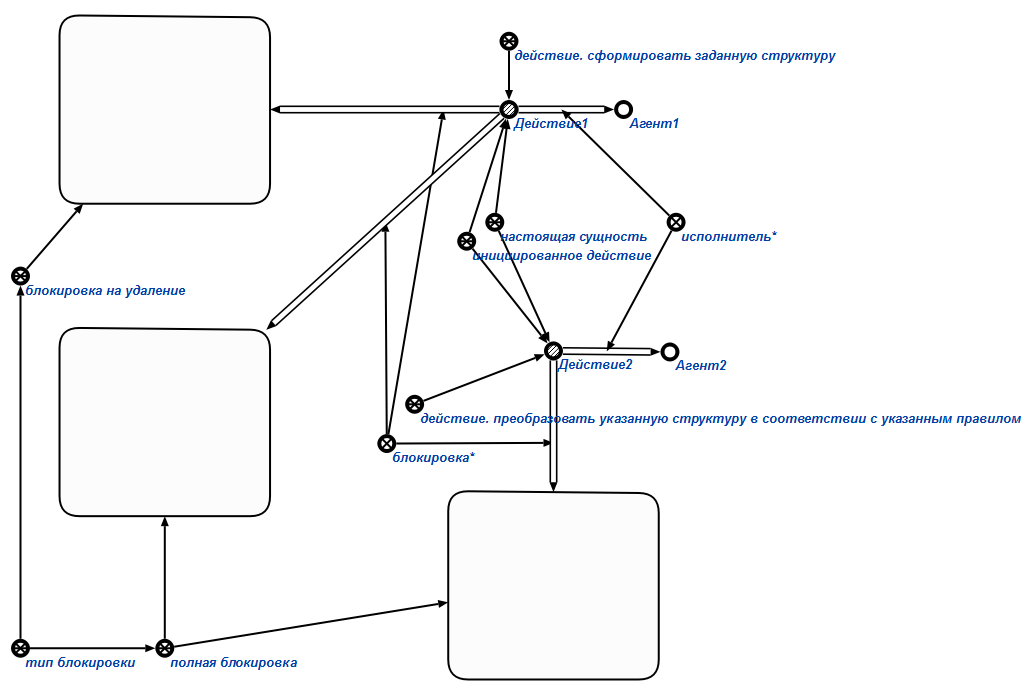
\includegraphics[width=1\linewidth]{figures/sd_agents/lock.png}
\end{figure}
}}

\scnheader{тип блокировки}
\scnexplanation{Множество \textbf{\textit{тип блокировки}} содержит все возможные классы блокировок, т.е. \textit{sc-структуры}, содержащие \textit{sc-элементы}, заблокированные каким-либо \textit{sc-агентом} на время выполнения им некоторого \textit{действия в sc-памяти}.}
\scnhaselement{полная блокировка}
\scnhaselement{блокировка на любое изменение}
\scnhaselement{блокировка на удаление}

\scnheader{полная блокировка}
\scnexplanation{Каждая \textit{структура}, принадлежащая множеству \textbf{\textit{полная блокировка}} содержит \textit{sc-элементы}, просмотр и изменение (удаление, добавление инцидентных \textit{sc-коннекторов}, удаление самих \textit{sc-элементов}, изменение содержимого в случае файла) которых запрещены всем \textit{sc-агентам}, кроме собственно \textit{sc-агента}, выполняющего соответствующее данной структуре \textit{действие в sc-памяти}, связанное с ней отношением \textit{блокировка*}.

Для того, чтобы исключить возможность реализации \textit{sc-агентов}, которые могут внести изменения в конструкции, описывающие блокировки других \textit{sc-агентов}, все элементы этих конструкций, в том числе, сам знак \textit{структуры}, содержащей заблокированные \textit{sc-элементы} (принадлежащей как множеству \textbf{\textit{полная блокировка}}, так и любому другому \textit{типу блокировки}) и связки отношения \textit{блокировка*}, связывающие эту \textit{структуру} и конкретное \textit{действие в sc-памяти}, добавляются в \textbf{\textit{полную блокировку}}, соответствующую данному \textit{действию в sc-памяти}. Таким образом, каждой \textbf{\textit{полной блокировке}} соответствует петля принадлежности, связывающая ее знак с самим собой.}

\scnheader{блокировка на любое изменение}
\scnexplanation{Каждая \textit{структура}, принадлежащая множеству \textbf{\textit{блокировка на любое изменение}} содержит \textit{sc-элементы}, изменение (физическое удаление, добавление инцидентных \textit{sc-коннекторов}, физическое удаление самих \textit{sc-элементов}, изменение содержимого в случае файла) которых запрещено всем \textit{sc-агентам}, кроме собственно \textit{sc-агента}, выполняющего соответствующее данной структуре \textit{действие в sc-памяти}, связанное с ней отношением \textit{блокировка*}. Однако не запрещен просмотр (чтение) этих \textit{sc-элементов} любым \textit{sc-агентом}.}

\scnheader{блокировка на удаление}
\scnexplanation{Каждая \textit{структура}, принадлежащая множеству \textbf{\textit{блокировка на удаление}} содержит \textit{sc-элементы}, удаление которых запрещено всем \textit{sc-агентам}, кроме собственно \textit{sc-агента}, выполняющего соответствующее данной структуре \textit{действие в sc-памяти}, связанное с ней отношением \textit{блокировка*}. Однако не запрещен просмотр (чтение) этих \textit{sc-элементов} любым \textit{sc-агентом}, добавление инцидентных sc-коннекторов.}

\scnheader{блокировка*}
\scnrelfromset{принципы работы}{
	\scnfileitem{в каждый момент времени одному процессу в sc-памяти может соответствовать только одна блокировка каждого типа};
	\scnfileitem{в каждый момент времени одному процессу в sc-памяти может соответствовать только одна блокировка, установленная на некоторый конкретный sc-элемент};
	\scnfileitem{при завершении выполнения любого процесса в sc-памяти все установленные им блокировки автоматически снимаются};
	\scnfileitem{для повышения эффективности работы системы в целом каждый процесс должен в каждый момент времени блокировать минимально необходимое множество sc-элементов, снимая блокировку с каждого sc-элемента сразу же, как это становится возможным (безопасным)};
	\scnfileitem{В случае когда в рамках \textit{процесса в sc-памяти} явно выделяются более частные подпроцессы (при помощи отношений \textit{темпоральная часть*, поддействие*, декомпозиция действия*} и т. д.), то каждый такой подпроцесс с точки зрения синхронизации выполнения рассматривается как самостоятельный процесс, которому в соответствие могут быть поставлены все необходимые блокировки.}
	\scnaddlevel{1}
	\scnrelfromlist{детализация}{
	\scnfileitem{все дочерние процессы в sc-памяти имеют доступ к блокировкам родительского процесса так же, как если бы это были блокировки соответствующие каждому из таких дочерних процессов};
	\scnfileitem{в свою очередь, родительский процесс не имеет какого-либо привилегированного доступа к sc-элементам, заблокированным дочерними процессами, и работает с ними так же, как любой другой процесс в sc-памяти. Исключение составляют sc-элементы, обозначающие сами дочерние процессы, поскольку родительский процесс должен иметь возможность управления дочерним, например, приостановки или прекращения их выполнения};
	\scnfileitem{все дочерние процессы по отношению друг к другу работают так же, как и по отношению к любым другим процессам};
	\scnfileitem{в случае, когда родительский процесс приостанавливает выполнение (становится \textit{отложенным действием}), \uline{все} его дочерние процессы также приостанавливают выполнение. В свою очередь, приостановка одного из дочерних процессов в общем случае не инициирует явно остановку всего родительского процесса и соответственно других дочерних.} 	
}
	\scnaddlevel{-1}
}

\scnheader{полная блокировка}
\scnrelfromset{принципы работы}{
	\scnfileitem{если sc-элемент, инцидентный некоторому sc-коннектору, попадает в какую-либо полную блокировку, то сам этот sc-коннектор по умолчанию также считается заблокированным этой же блокировкой. Обратное в общем случае неверно, т. к. часть sc-коннекторов, инцидентных некоторому sc-элементу, может быть полностью заблокирована, при этом сам этот элемент заблокирован не будет. Такая ситуация типична, например, для sc-узлов, обозначающих классы понятий};
	\scnfileitem{каждый процесс в sc-памяти может свободно изменять или удалять любые sc-элементы, попадающие в полную блокировку, соответствующую этому процессу.}
}
\scnaddlevel{1}
	\scnnote{Принципы работы с \textit{полными блокировками}, с одной стороны, наиболее просты, поскольку все процессы, кроме установившего такую блокировку, не имеют доступа к заблокированным sc-элементам и конфликты возникнуть не могут. С другой стороны, частое использование блокировок такого типа может привести к тому, что система не сможет использовать в полной мере имеющиеся у нее знания и давать неполные или даже некорректные ответы на поставленные вопросы.}
\scnaddlevel{-1}


\scnheader{блокировка на любое изменение}
\scnrelfromset{принципы работы}{
	\scnfileitem{на один и тот же sc-элемент в один момент времени может быть установлена только одна блокировка одного типа, но разные процессы могут одновременно установить на один и тот же элемент блокировки двух разных типов. Это касается случая, когда первый процесс установил на некоторый sc-элемент блокировку на удаление, а второй процесс затем устанавливает блокировку на любое изменение. В других случаях возникает конфликт блокировок};
	\scnfileitem{установка блокировки любого типа также считается изменением, таким образом, если на некоторый sc-элемент была установлена блокировка на любое изменение, то другой процесс не сможет установить на этот же sc-элемент блокировку любого типа, пока первый процесс не снимет свою};
	\scnfileitem{если блокировка на удаление устанавливается на некоторый sc-коннектор, то по умолчанию та же блокировка устанавливается на инцидентные этому sc-коннектору sc-элементы, поскольку удаление этих элементов приведет к удалению этого коннектора.}
}
\scnaddlevel{1}
	\scnrelto{принципы работы}{блокировка на удаление}
\scnaddlevel{-1}

\scnheader{процесс в sc-памяти}
\scnidtf{действие в sc-памяти}
\scnrelfrom{разбиение}{Классификация процессов в sc-памяти с точки зрения синхронизации их выполнения}
\scnaddlevel{1}
	\scneqtoset{действие поиска sc-элементов;действие генерации sc-элементов;действие удаления sc-элементов;действие установки блокировки некоторого типа на некоторый sc-элемент;действие снятия блокировки с некоторого sc-элемента}
\scnaddlevel{-1}

\scnheader{транзакция в sc-памяти}
\scnexplanation{В некоторых случаях для того, чтобы обеспечить синхронизацию, необходимо объединять несколько элементарных действий над sc-памятью в одно неделимое действие (\textit{транзакцию в sc-памяти}), для которого гарантируется, что ни один сторонний процесс не сможет прочитать или изменить участвующие в этом действии sc-элементы, пока действие не завершится. При этом, в отличие от ситуации с полной блокировкой, процесс, пытающийся получить доступ к таким элементам, не продолжает выполнение так, как если бы этих элементов просто не было в sc-памяти, а ожидает завершения транзакции, после чего может выполнять с данными элементами любые действия согласно общим принципам синхронизации процессов. Проблема обеспечения транзакций не может быть решена на уровне SC-кода и требует реализации таких неделимых действий на уровне \textit{платформы интерпретации sc-моделей}.}

\scnheader{действие поиска sc-элементов}
\scnexplanation{В случае осуществления поиска все найденные и сохраненные в рамках какого-либо процесса sc-элементы попадают в соответствующую данному процессу \textit{блокировку на любое изменение}. Таким образом, гарантируется целостность фрагмента базы знаний, с которым работает некоторый процесс в sc-памяти. При этом поиск и автоматическая установка такой блокировки должны быть реализованы как \textit{транзакция в sc-памяти}.

Такой подход также позволяет избежать ситуации, когда один процесс заблокировал некоторый sc-элемент на любое изменение, а второй процесс пытается сгенерировать или удалить \textit{sc-коннектор}, инцидентный данному \textit{sc-элементу}. В таком случае второй процесс должен будет предварительно найти и заблокировать указанный \textit{sc-элемент} на любое изменение, что вызовет конфликт блокировок (\textit{взаимоблокировку*}).}

\scnheader{действие генерации sc-элементов}
\scnexplanation{В случае генерации любого sc-элемента в рамках некоторого процесса он автоматически попадает в полную блокировку, соответствующую данному процессу. При этом генерация и автоматическая установка такой блокировки должны быть реализованы как \textit{транзакция в sc-памяти}. При необходимости сгенерированные элементы могут быть удалены (т. е. их временное существование вообще никак не отразится на деятельности других процессов) или разблокированы в случае, когда сгенерирована информация, которая может иметь некоторую ценность в дальнейшем.}

\scnheader{действие установки блокировки некоторого типа на некоторый sc-элемент}
\scnexplanation{В случае если какой-либо процесс пытается установить блокировку любого типа на какой-либо sc-элемент, уже заблокированный каким-либо другим процессом, то, с одной стороны, блокировка не может быть установлена, пока другой процесс не разблокирует указанный sc-элемент; с другой стороны, для того чтобы обеспечить возможность поиска и устранения \textit{взаимоблокировок}, необходимо явно указывать тот факт, что какой-либо процесс хочет получить доступ к какому-либо заблокированному другим процессом sc-элементу. Для того чтобы иметь возможность указать, какие процессы пытаются заблокировать уже заблокированный \textit{sc-элемент}, предлагается наряду с отношением \textit{блокировка*} использовать отношение \textit{планируемая блокировка*}, полностью аналогичное отношению \textit{блокировка*}.

Описанный механизм регулирует также и процессы поиска, поскольку поиск и сохранение некоторого sc-элемента предполагает установку \textit{блокировки на любое изменение}. Кроме того, следует учитывать, что на один sc-элемент \textit{блокировка на любое изменение} может быть установлена после \textit{блокировки на удаление}, соответствующей другому процессу. В этом случае использовать отношение \textit{планируемые блокировки*} нет необходимости.}
\scnnote{Действие проверки наличия на некотором sc-элементе блокировки и в зависимости от результата проверки, установки блокировки или планируемой блокировки (с указанием приоритета при необходимости) должно быть реализовано как транзакция.}

\scnheader{планируемая блокировка*}
\scnsubset{блокировка*}
\scnexplanation{Процесс, которому в соответствие поставлена \textit{планируемая блокировка*}, приостанавливает выполнение до тех пор, пока уже установленные блокировки не будут сняты, после чего \textit{планируемая блокировка*} становится реальной \textit{блокировкой*} и процесс продолжает выполнение в соответствии с общими правилами.}

\scnheader{приоритет блокировки*}
\scnrelfrom{область определения}{планируемая блокировка*}
\scnexplanation{В случае, когда на один и тот же sc-элемент планируют установить блокировку сразу несколько процессов, используется отношение \textit{приоритет блокировки*}, связывающее между собой пары отношения \textit{планируемая блокировка*}. Как правило, приоритет блокировки определяется тем, какой из процессов раньше попытался установить блокировку на рассматриваемый sc-элемент, хотя в общем случае приоритет может устанавливаться или меняться в зависимости от дополнительных критериев.}

\scnheader{действие удаления sc-элементов}
\scnnote{В случае попытки удаления некоторого sc-элемента некоторым процессом удаление может быть осуществлено только в случае, когда на данный sc-элемент не установлена (и не планируется) ни одна блокировка каким-либо другим процессом.
	
В других случаях необходимо обеспечить корректное завершение выполнения всех процессов, работающих с данным sc-элементом, и только потом удалить его физически.
	
Для реализации такой возможности каждому процессу в соответствие может быть поставлено множество удаляемых данным процессом sc-элементов.}
\scnnote{Действие проверки наличия блокировок или планируемых блокировок на удаляемый sc-элемент и собственно его удаление или добавление во множество удаляемых sc-элементов для соответствующего процесса должно быть реализовано как транзакция.}

\scnheader{удаляемые sc-элементы*}
\scnrelfrom{первый домен}{процесс в sc-памяти}
\scnexplanation{Sc-элементы, попавшие во множество удаляемых sc-элементов некоторого процесса в sc-памяти, доступны процессам, уже установившим (или планирующим установить) на эти sc-элементы блокировки ранее (до попытки его удаления), а для всех остальных процессов эти sc-элементы уже считаются удаленными. Процесс, пытающийся удалить sc-элемент, приостанавливает свое выполнение до того момента, пока все заблокировавшие и планирующие заблокировать данный sc-элемент процессы не разблокируют его. В общем случае один sc-элемент может входить во множества удаляемых элементов одновременно для нескольких процессов, в этом случае все такие процессы одновременно продолжат выполнение после снятия с этого sc-элемента всех блокировок. Если удаление пытается осуществить один из процессов, уже установивший на указанный sc-элемент блокировку, то алгоритм действий остается прежним -- sc-элемент добавляется во множество удаляемых данным процессом sc-элементов, и будет физически удален, как только все остальные процессы, установившие на данный sc-элемент блокировки, снимут их.}

\scnheader{действие снятия блокировки с некоторого sc-элемента}
\scnrelfromvector{алгоритм выполнения}{\scnfileitem{если на данный sc-элемент установлена одна или несколько \textit{планируемых блокировок*}, то первая из них по приоритету (или единственная) становится \textit{блокировкой*}, соответствующий ей процесс продолжает выполнение (становится настоящей сущностью); связка отношения приоритет выполнения, соответствовавшая удаленной связке отношения \textit{планируемая блокировка*} также удаляется, т. е. приоритет смещается на одну позицию};
\scnfileitem{если \textit{планируемых блокировок*}, установленных на данный sc-элемент, нет, но он попадает во множество удаляемых sc-элементов для одного или нескольких процессов, то рассматриваемый sc-элемент физически удаляется, а приостановленные до его удаления процессы продолжают свое выполнение (становится настоящими сущностями)};
\scnfileitem{если на данный sc-элемент не установлены планируемые блокировки и он не входит во множество удаляемых для какого-либо процесса, то блокировка просто снимается без каких-либо дополнительных изменений.}}

\scnheader{транзакция в sc-памяти}
\scnsubdividing{поиск некоторой конструкции в sc-памяти и автоматическая установка блокировки на любое изменение на найденные sc-элементы;генерация некоторого sc-элемента и автоматическая установка на него полной блокировки;проверка наличия на некотором sc-элементе блокировки и в зависимости от результата проверки установка блокировки или планируемой блокировки;проверка наличия блокировок или планируемых блокировок на удаляемый sc-элемент и собственно его удаление или добавление во множество удаляемых sc-элементов для соответствующего процесса;снятие блокировки с заданного sc-элемента и при необходимости установка первой по приоритету планируемой блокировки или удаление данного sc-элемента, если он входит во множество удаляемых sc-элементов для некоторого процесса;поиск подпроцессов процесса и добавление их во множество отложенных действий в случае добавления самого процесса в данное множество;поиск подпроцессов процесса и удаление их из множества отложенных действий в случае удаления самого процесса из данного множества}

\scnheader{абстрактный программный sc-агент}
\scnnote{При реализации \textit{абстрактных программных sc-агентов} на \textit{языке SCP}, соблюдение всех принципов синхронизации соответствующих этим sc-агентам процессов обеспечивается на уровне \textit{sc-агентов интерпретации scp-программ}, т. е. средствами \textit{платформы интерпретации sc-моделей}. При реализации \textit{абстрактных программных sc-агентов} на уровне платформы, соблюдение всех принципов синхронизации возлагается, во-первых, непосредственно на разработчика агентов, во-вторых, -- на разработчика платформы. Так, например, платформа может предоставлять доступ к хранимым в sc-памяти элементам через некоторый программный интерфейс, уже учитывающий принципы работы с блокировками, что избавит разработчика агентов от необходимости учитывать все эти принципы вручную.}
\scnrelfromset{принципы работы}{\scnfileitem{в результате появления в sc-памяти некоторой конструкции, удовлетворяющей условию инициирования какого-либо \textit{абстрактного sc-агента}, реализованного при помощи \textit{Языка SCP}, в \textit{sc-памяти} генерируется и инициируется \textit{scp-процесс}. В качестве шаблона для генерации используется \textit{агентная scp-программа}, соответствующая данному \textit{абстрактному sc-агенту}.};
\scnfileitem{каждый такой \textit{scp-процесс}, соответствующий некоторой \textit{агентной \mbox{scp-программе}}, может быть связан с набором структур, описывающих блокировки различных типов. Таким образом, синхронизация взаимодействия параллельно выполняемых \textit{scp-процесcов} осуществляется так же, как и в случае любых других \textit{действий в sc-памяти}.};
\scnfileitem{несмотря на то что каждый \textit{scp-оператор} представляет собой атомарное действие в sc-памяти, являющееся поддействием в рамках всего \textit{\mbox{scp-процесса}}, блокировки, соответствующие одному оператору, не вводятся, чтобы избежать громоздкости и избытка дополнительных системных конструкций, создаваемых при выполнении некоторого \textit{scp-процесса}. Вместо этого используются блокировки, общие для всего \textit{scp-процесса}. Таким образом, \textit{агенты интерпретации scp-программ} работают только с учетом блокировок, общих для всего интерпретируемого \textit{scp-процесса}.};
\scnfileitem{процессы, описывающие деятельность агентов интерпретации \textit{scp-программ}, как правило, не создаются, следовательно, и не вводятся соответствующие им блокировки. Поскольку такие агенты работают с уникальным scp-процессом и их число ограничено и известно, то использование блокировок для их синхронизации не требуется.};
\scnfileitem{в случае приостановки \textit{scp-процесса} (добавления его во множество \textit{отложенных действий}) в соответствии с общими правилами синхронизации все его дочерние процессы также должны быть	приостановлены. В связи с этим все \textit{scp-операторы}, которые в	этот момент являются \textit{настоящими сущностями}, становятся	\textit{отложенными действиями}.};
\scnfileitem{во избежание нежелательных изменений в самом теле \textit{scp-процесса}, вся конструкция, сгенерированная на основе некоторой \textit{scp-программы} (весь \textit{sc-текст}, описывающий декомпозицию \textit{scp-процесса} на \textit{scp-операторы}), должна быть добавлена в \textit{полную блокировку}, соответствующую данному \textit{scp-процессу}.};
\scnfileitem{при необходимости разблокировать или заблокировать некоторую конструкцию каким-либо типом блокировки используются соответствующие \textit{scp-операторы} класса \textit{scp-оператор управления блокировками}.};
\scnfileitem{после завершения выполнения некоторого scp-процесса его текст, как правило, удаляется из \textit{sc-памяти}, а все заблокированные конструкции освобождаются (разрушаются знаки структур, обозначавших блокировки).};
\scnfileitem{как правило, частный \textit{класс действий}, соответствующий конкретной \textit{scp-программе}, явно не вводится, а используется более общий класс \textit{scp-процесс}, за исключением тех случаев, когда введение	специального \textit{класса действий} необходимо по каким-либо другим соображениям.}}
	
\scnheader{блокировка*}
\scnnote{В общем случае весь механизм блокировок может описываться как на уровне SC-кода (для повышения уровня платформенной независимости), так и при необходимости может быть реализован на уровне \textit{платформы интерпретации sc-моделей}, например для повышения производительности. Для этого каждому выполняемому в sc-памяти процессу на нижнем уровне может быть поставлена в соответствие некая уникальная таблица, в каждый момент времени содержащая перечень заблокированных элементов с указанием типа блокировки.}

\scnheader{взаимоблокировка*}
\scnexplanation{В зависимости от конкретных \textit{типов блокировок} установленных паралельно выполняемыми процессами на некоторые sc-элементы и того, какие конкретно действия с этими \textit{sc-элементами} предполагается выполнить далее в рамках выполнения этих процессов, возможны ситуации взаимоблокировки, когда каждый из указанных процессов будет ожидать снятия блокировки вторым процессом с нужного \textit{sc-элемента}, не снимая при этом установленной им самим блокировки с \textit{sc-элемента}, доступ к которому необходим второму процессу.
	
В случае когда хотя бы одна из блокировок является \textit{полной блокировкой}, ситуация взаимоблокировки возникнуть не может, поскольку \textit{sc-элементы}, попавшие в \textit{полную блокировку} некоторого \textit{scp-процесса}, не доступны другим \textit{scp-процессам} даже для чтения и, таким образом, остальные \textit{scp-процессы} будут работать так, как будто заблокированные \textit{sc-элементы} просто отсутствуют в текущем состоянии \textit{sc-памяти}.
	
В случаях, когда ни одна из установленных блокировок не является \textit{полной блокировкой}, возможно появление взаимоблокировок.}
\scnnote{Устранение \textit{взаимоблокировки} невозможно без вмешательства специализированного \textit{sc-метаагента}, который имеет право игнорировать блокировки, установленные другими процессами. 

В общем случае проблема конкретной взаимоблокировки может быть решена путем выполнения специализированным \textit{sc-метаагентом} следующих шагов:	
\begin{scnitemize}
	\item откат нескольких операций, выполненных одним из участвующих в взаимоблокировке процессов настолько шагов назад, насколько это необходимо для того, чтобы второй процесс получил доступ к необходимым \textit{sc-элементам} и смог продолжить выполнение;
	\item ожидание выполнения второго процесса вплоть до завершения или до снятия им всех блокировок с \textit{sc-элементов}, доступ к которым необходимо получить первому процессу;
	\item повторное выполнение в рамках первого процесса отмененных операций и продолжение его выполнения, но уже с учетом изменений в памяти, внесенных вторым процессом.		
\end{scnitemize}
}

\scnheader{sc-метаагент}
\scnexplanation{Для \textit{sc-метаагентов} все sc-элементы, в том числе описывающие блокировки, планируемые блокировки и т. д. полностью эквивалентны между собой с точки зрения доступа к ним, т. е. любой \textit{sc-метаагент} имеет доступ к любым sc-элементам, даже попавшим в полную блокировку для какого-либо другого процесса. Это необходимо для того, чтобы \textit{sc-метаагенты} смогли выявлять и устранять различные проблемы, например, описанную выше проблему взаимоблокировки.
	
Таким образом, проблема синхронизации деятельности \textit{sc-метаагентов} требует введения дополнительных правил.
	
Указанную проблему разделим на две более частные:
\begin{scnitemize}
	\item обеспечение синхронизации деятельности \textit{sc-метаагентов} между собой;
	\item обеспечение синхронизации деятельности \textit{sc-метаагентов} и \textit{программных sc-агентов}.		
\end{scnitemize}
	
Первую проблему предлагается решить за счет запрета параллельного выполнения \textit{sc-метаагентов}. Таким образом, в каждый момент времени в рамках одной \textit{ostis-системы} может существовать только один процесс, соответствующий \textit{sc-метаагенту} и являющийся \textit{настоящей сущностью}. 
	
Вторую проблему предлагается решить за счет введения дополнительных привилегий для \textit{sc-метаагентов} при обращении к какому-либо sc-элементу. Для этого достаточно одного правила: 

Если некоторый sc-элемент стал использоваться в рамках процесса, соответствующего \textit{sc-метаагенту} (например, стал элементом хотя бы одного scp-оператора, входящего в данный процесс), то все процессы, в блокировки соответствующие которым попадает указанный sc-элемент, становятся отложенными действиями (приостанавливают выполнение). Как только указанный sc-элемент перестает использоваться в рамках процесса, соответствующего \textit{sc-метаагенту}, все приостановленные по этой причине процессы продолжают выполнение.
	
Рассмотренные ограничения не ухудшают производительность ostis-системы существенно, поскольку \textit{sc-метаагенты} предназначены для решения достаточно узкого класса задач, которые, как показал опыт практической разработки прототипов различных \textit{ostis-систем}, возникают достаточно редко.}
\scnnote{Стоит отметить, что возможна ситуация, при которой выполнение некоторого процесса в sc-памяти прервано по причине возникновения какой-либо ошибки. В таком случае существует вероятность того, что блокировка, установленная данным процессом не будет снята до тех пор, пока этого не сделает sc-метаагент, обнаруживший подобную ситуацию. Однако указанная проблема на уровне sc-модели может быть решена лишь частично, для случаев, когда ошибка возникает при интерпретации scp-программы, отслеживается scp-интепретатором и в памяти формируется соответствующая конструкция, сообщающая о проблеме sc-метаагенту. Случаи, когда возникла ошибка на уровне scp-интерпретатора или sc-хранилища, должны рассматриваться на уровне платформы интерпретации sc-моделей.}

\bigskip
\scnendstruct

\bigskip
\scnendstruct \scnendcurrentsectioncomment

\end{SCn}